\documentclass{article}
\usepackage[utf8]{inputenc}
\usepackage{amsmath}
\usepackage{mathtools}
\usepackage{bm}
\usepackage{graphicx}
\title{COL352: Assignment 2}
\author{Sachin 2019CS10722 }
\date{February, 2022}

\begin{document}

\maketitle


\section{Question 1}
Let L = $\{ bin(p) : $ p is prime $\}$\\

Proving by updated version of pumping lemma.\\
So we need to show:-\\
$\forall n \geq 0$\\
$\exists \text{ } p = uwv \in L : |w| \geq n$\\
$\forall xyz \in \Sigma^* : xyz = w, |xy| \leq n, |y| > 0$\\
$\exists i \geq 0 : uxy^izv \notin L$\\

Let $p = 2^{n+1} + 1$\\
$v = 1$\\
$w = $ 2nd bit to nth bit of p $=> w = 0....0 $ n times\\
u = remaining part of p\\

Now, since w is all zero, any split xyz of w will just differ in their number of zeros. \\
Let, $|x| = r, |y| = s, |z| = t : r+s \leq n, s > 0$\\
$=> r+s+t = n$\\
$p' = uxy^izv = 2^{r+is+t+1} + 1$\\
$r+is+t+1 = r+s+t + (i-1)s + 1 = n + (i-1)s + 1$\\
$=> p' = 2^{n+1+(i-1)s} + 1$\\
$=> p' = 2^{n+1}2^{(i-1)s} + 1$\\
$=> p' = (p-1)2^{(i-1)s} + 1$  \\
$=> p' = p2^{(i-1)s} - (2^{(i-1)s} - 1)$\\
take i = p\\
$=> p' = p2^{(p-1)s} - (2^{(p-1)s} - 1)$\\
We, know that for any prime number $p : a^{p-1} mod p = 1$ (done in course col351, fermat's little theorem)\\
$=> 2^{p-1} mod p = 1 => 2^{(p-1)s} mod p = 1 => 2^{(p-1)s} - 1 (mod p) = 0$\\
$=> $ second term is divisible by p then let it be p*k\\
$=> p' = p (2^{(p-1)s} - k)$\\
$=> p' $ is divisible by p, hence not prime and hence not in L\\


\pagebreak


\section{Question 2}
\textbf{The n-th Fibonacci number is defined as \boldsymbol{$F_1 = 1, F_2 = 1$}, and for all \boldsymbol{$n \geq 3$}, \boldsymbol{$F_n = F_{n-1} + F_{n-2}$} .Consider the language over \boldsymbol{$\Sigma = \{a\}$ $L_2 = \{a^m | m = F_n \}$} Is \boldsymbol{$L_2$} regular? Justify your answer.}\\
\newline
The given language is not regular and we will prove this using the pumping lemma. \\
\textbf{To Prove:} $L_2$ is not regular.\\
\textbf{Proof:} We will use the contrapositive of the pumming lemma here. So let k be the pumping length s.t. $k\geq 1$. Now we pick a fibonacci number $F_n\geq k$ and also $F_{n+1}-F_{n}>k$. Such a fibonacci number exists clearly because second condition basically comes to $F_{n-1}>k$. So we have to find a fibonacci number which is greater than k and the fibonacci just number before it is also grater than k. That is clearly possible since fibonacci is a fast growing series.\\
Now,
\[ k\geq 1 , a^{F_n}\in L_2 \ and \ |a^{F_n}|\geq k\] 
Every break up of $a^{F_n}$ can be written as xyz :
\[x=a^r,y=a^s,z=a^t\ where \ r+s+t=F_n\] 
\[ Also, \ |xy|\leq k \ and \ y\neq \epsilon \implies  s\neq0 \ and \ s\leq k\ \ \ \ \ \ \ \  -(i)\]
Now consider i=2 . Clearly  $i\geq0$.
We can pump up y for i=2 to get:
\[xy^2z = a^{r+2*s+t}\] 
\[=> a^{F_n+s}\] 
\[We \ know \ F_n<F_n+s\leq F_n+k<F_{n+1} \ \ \ \ \ - From\ (i)\]
So we have shown that $F_n+s$ is not a fibonacci number so $xy^2z\notin L_2$ . Hence by the contrapositive of the pumping lemma $L_2$ is not a regular language. Hence Proved.

\pagebreak



\section{Question 3}
\textbf{If A is any language, let $A_{\frac{1}{2}-}$ denote the set of all first halves of strings in A so that \[ A_{\frac{1}{2}-} = \text{\{x \boldsymbol{$|$} for some \boldsymbol{$y,|x|=|y|$} and xy} \in A\} \] 
        Show that if A is regular, then so is \boldsymbol{$A_{\frac{1}{2}-}$}.\\}

To, show that $A_{\frac{1}{2}-}$ is regular, it is sufficient to show that there exist a 2DFA that accepts $A_{\frac{1}{2}-}$ (as it was proved in class that language accepted by 2DFA is regular).\\
Now, before constructing the 2DFA, consider the following psuedo code:- \\

Let DFA D accepts A, and $x \in \Sigma^*$
Start from start state of D\\
Run the string x on D\\
Suppos final state is $q_i$\\
From, $q_i$ at each step traverse to all states having 1-step transition from $q_i$\\
Iteratively, make similar transitions from all states at step i\\
Perform $|x|$ such steps\\
If out of all states in last step if any of them is in final state then x is accepted else x is rejected.\\

So, basically from state $q_i$ we are traversing all states that are $|x|$ transitions away (hence got all possible final states that we can get after running $xy$ such that $|x| = |y|$).\\
Since $\hat{\delta}(q_0,xy) = \hat{\delta}(\hat{\delta}(q_0,x),y)$\\

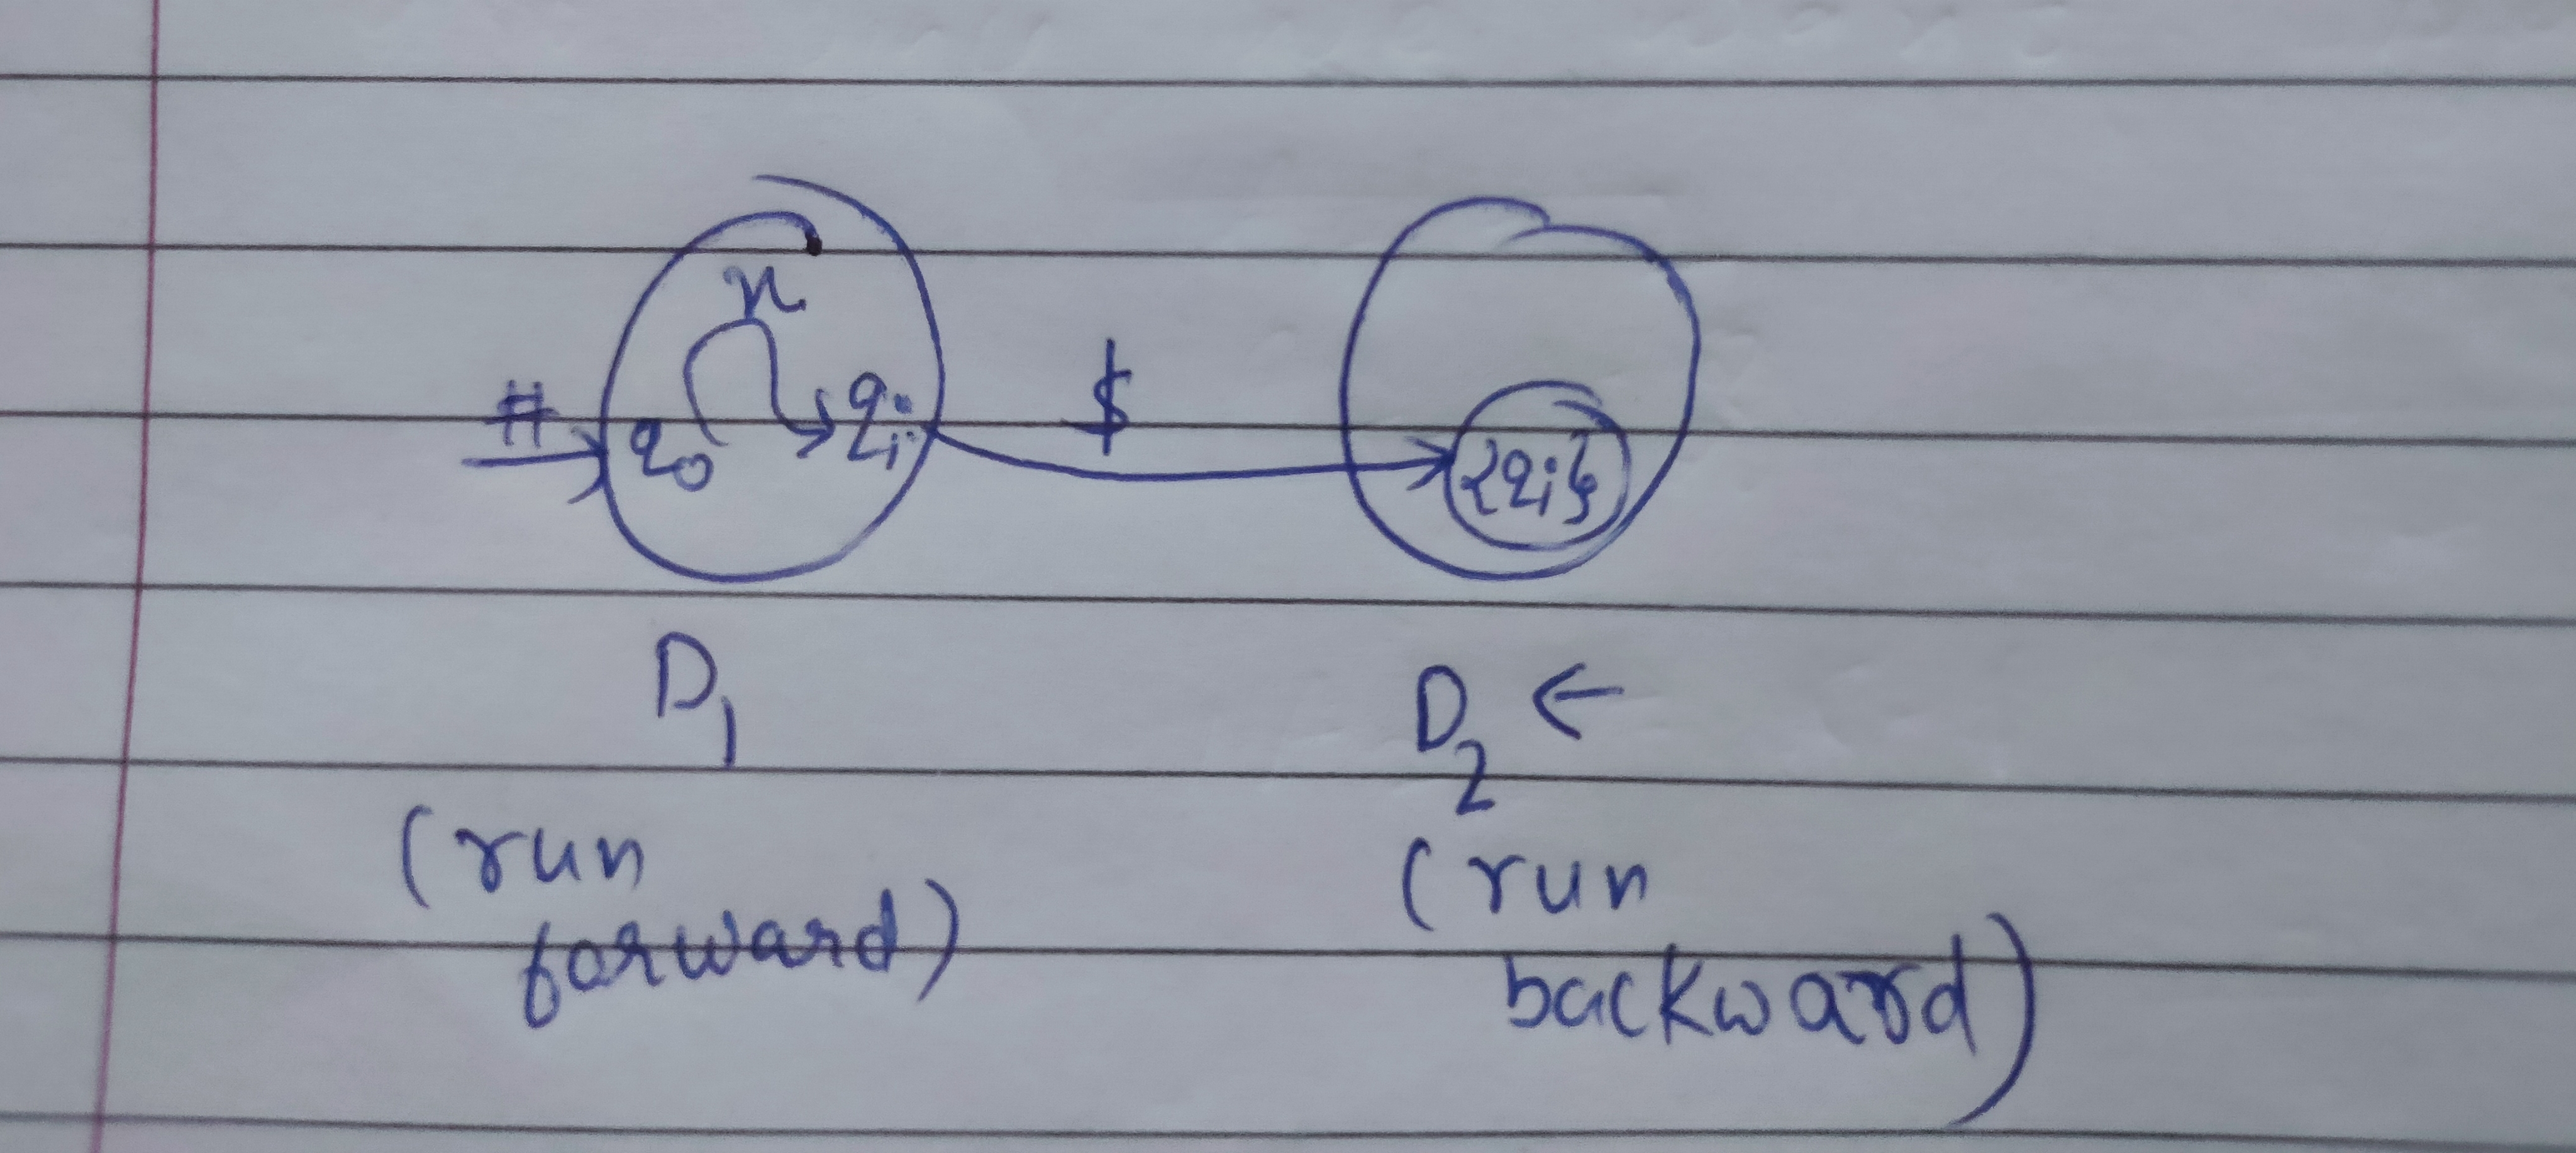
\includegraphics[width=13cm]{3.jpg}\\

Now, lets folmally define the 2DFA D' that runs above psuedo code:- 
We will require 2 DFA's D1 and D2 to construct D'.\\
Let D1 = D = $\{Q,\Sigma,\delta,q_0,F\}$\\
First run of x would be on D with transition function $\delta$ and moving right.\\
Second run would be on D2 = $\{2^Q,\Sigma,\delta_1,q_0,F'\}$ with transition function $\delta'$ and moving left.\\

So, D' = $\{Q',\Sigma \bigcup \{ \#,\$ \},\delta',q_0,q_a,q_r\}$\\ is defined as:- 
$Q' = Q \bigcup 2^Q \bigcup q_a \bigcup q_r$\\
$\delta'(q'_i,a) $ defined as:
\begin{enumerate}
    \item $q'_i \in Q$ (first run)\\
    $\delta'(q_0,\#) = (q_0,R)$\\
    $\delta'(q_i,c) = (\delta(q_i,c),R)$ if $c \in \Sigma$\\
    $\delta'(q_i,\$) = (\{q_r\},L)$\\

    \item $q'_i \in 2^Q$ (second run)\\
    $\delta'(q'_i,c) = ( \bigcup\limits_{q_k \in q'_i} \{ \bigcup\limits_{a \in \Sigma} \delta(q_i,a) \},L)$ if $c \in \Sigma$\\
    $\delta'(q'_i,\#) = (q_a,L)$ if $q'_i \bigcap F \neq \phi$\\
    $\delta'(q'_i,\#) = (q_r,L)$ if $q'_i \bigcap F = \phi$\\
\end{enumerate} 

\textbf{Claim: } Above 2DFA accepts $A_{\frac{1}{2}-}$\\
\textbf{Proof:}     
    Consider string $x \in \Sigma^*$\\
    if, $x \in A_{\frac{1}{2}-}$\\
    $<=> \exists y$ such that $ xy \in A, |x| = |y| = $ n(say)\\
    Consider the run of $xy$ on D.\\
    Let, $\hat{\delta}(q_0,x) = q_i $
    $\hat{\delta}(q_i,y) = q_j$\\
    $<=> q_j \in F$\\
    Now, consider the run of x on D' \\
    $(q_0,0) \xrightarrow{x} (q_i,n) $\\
    $(q_i,n) \xrightarrow{y} (q'_i,2n) $\\
    $q'_i$ is the set of all possible final states rechable from $q_i$ after n transition\\
    Clearly $q_j$ is in $q'_i$ (as $|y| = n$)\\
    $=> q_j \in F <=> q'_i \bigcup F \neq \phi$ \\
    $x \in A_{\frac{1}{2}-} <=> x $ accepted by D'\\
    Hence $L(D') = A_{\frac{1}{2}-}$\\
    Hence done. 
\pagebreak




\section{Question 4}
\textbf{If A is any language, let \boldsymbol{$A_{\frac{1}{3}-\frac{1}{3}}$} denote the set of strings in A with the middle-third removed so that
         \[A_{\frac{1}{3}-\frac{1}{3}} = \text{ \{ xz \boldsymbol{$|$} for somey, \boldsymbol{$|x|=|y|=|z|$} and \boldsymbol{$xz \in A$} \}} \]
         Show that if A is regular, then \boldsymbol{$A_{\frac{1}{3}-\frac{1}{3}}$} is not necessarily regular.\\}

To disprove the that $A_{\frac{1}{3}-\frac{1}{3}}$ is not necessarily regular if A is regular we will show a couter-example. That is we need a regular language A 
such that $A_{\frac{1}{3}-\frac{1}{3}}$ is not regular. \\
Consider the regular language $A = a^*bc^*$ .\\
\paragraph{}
\textbf{Claim: } $A_{\frac{1}{3}-\frac{1}{3}}$ is not regular.\\
\textbf{Proof: \\}
Proving this via contradiction.\\
Suppose $A_{\frac{1}{3}-\frac{1}{3}}$ is regular.\\
Now, consider the following language made by intersection of $A$ and $A_{\frac{1}{3}-\frac{1}{3}}$ :\\
$L = A_{\frac{1}{3}-\frac{1}{3}} \text{ } \bigcap \text{ } a^*c^* $\\

\textbf{Claim : } $L$ is not regular.\\
\textbf{Proof: }\\
Any string x in A is of the form $a^n b c^m : n,m \geq 0$.\\
So, for any string s of $A_{\frac{1}{3}-\frac{1}{3}}$ following cases are possible: -

\begin{enumerate}
    \item \textbf{Case 1: } $s = a^{k_1}c^{k_2}$ where $k_1,k_2 > 0 \& k_1 = k_2$\\
        This would be the case when b is not in middle third\\
        Proving $k_1 = k_2$\\
        Since, b is not in middle third, hence $a^{k_1}$ and $c^{k_2}$ comes from first third and last third respectively.\\
        And by the defination of $A_{\frac{1}{3}-\frac{1}{3}}$ we have $|a^{k_1}| = |c^{k_2}| => k_1 = k_2$\\
        $=> s = a^kc^k$
    \item \textbf{Case 2: } $s = a^{k_1}bc^{k_2}$ where $k_1,k_2 \geq 0$\\
    This would be the case when b is in middle third\\
\end{enumerate}

Now, $L = A_{\frac{1}{3}-\frac{1}{3}} \text{ } \bigcap \text{ } a^*c^* $\\
In intersection only first case of s will be considered since b cannot be in second language of intersection.\\
Hence $L = \{ \bigcup {s \text{ from case 1}} \text{ } \} \bigcap \text{ } a^*c^* = \{a^nc^n \forall n \geq 0 \}$ \\
Clearly L is irregular (provved in class).\\
But L is intersection of 2 regular languages and has to regular by closure of regularity.\\
That is a contradiction.\\
Hence our assumption that $A_{\frac{1}{3}-\frac{1}{3}}$ is regular is false.\\
Hence proved.

\pagebreak


\section{Question 5}


\pagebreak

\section{Question 6}
\textbf{Let M = \boldsymbol{$(Q, \Sigma, q_0 , \delta, F )$} be a DFA and let h be a state of M called its “home”. A synchronizing
sequence for M and h is a string \boldsymbol{$s\in \Sigma^{*}$} where \boldsymbol{$\delta(q,s)$} = h for every \boldsymbol{$q\in Q$}. Say that M
is synchronizable if it has a synchronizing sequence for some state h. Prove that if M is a
k-state synchronizable DFA, then it has a synchronizing sequence of length at most \boldsymbol{$q^3$} . Can you improve upon this bound?} \\
\newline
\textbf{Given:} We have a DFA M=$(Q, \Sigma, q_0 , \delta, F )$ which is synchronizable according to the definition given above. Also let us suppose k=$|Q|$ i.e. k is the number of states of the DFA. $h\in Q$ be the home state of M and $s\in\Sigma^{*}$\\ be the synchronizing sequence.\\ 
\textbf{To Prove:} The upper bound of the synchronizing sequence is $k^3$.\\
\textbf{Proof:} If we choose any two states $q_1\in Q$ and $q_2\in Q$ such that $q_1 \neq q_2$ then there must exist a sequence of alphabet lets call it $s^{'}$ that takes both $q_1$ and $q_2$ to the same state. So $\delta^{'}(q_1,s^{'})=\delta^{'}(q_2,s^{'})$. This holds because the DFA is synchronizable.\\
Now the length of the smallest $s^{'}$ such that the above condition is met is at max k*(k-1). This can be proved through the piegon hole principle. Suppose the length of $s^{'}$ is greater than k*(k-1). But we know that size of set of pair of distinct states is k*(k-1). So that would mean that some pair of states is repeated i.e. $\delta^{'}(q_1,s_1s_2...s_i)$=a , $\delta^{'}(q_2,s_1s_2....s_i)$=b and $\delta^{'}(q_1,s_1s_2....s_j)$=a , $\delta^{'}(q_2,s_1s_2....s_j)=b$ where $j>i$ and $s^{'}$=$s_1s_2....s_n$. But since the states are repeated we can omit the alphabet between $s_i$ and $s_j$ and there would be no difference. But that is contradiction because because $s^{'}$ was of the least length. So that proves that length of the string $s^{'}$ is at most $k*(k-1)$. \\
Now if we run $s^{'}$ we have found on all the states of Q then it would lead us to at most k-1 distinct states. This is true because of the way we constructed $s^{'}$ $q_1$ and $q_2$ would lead to same state. Now we will apply this process recursively for smaller number of states till the number of states reach 1. Let the state that was left be $h^{'}$ and the concatination of all the $s^{'}$ obtained  at each recursive step be $s^{''}$. \\
We can say that $s=s^{''}$ and $h=h^{'}$ because the way we have constructed $s^{''}$ and $h^{'}$, every state will reach $h^{'}$ if applied $s^{''}$. So $s^{''}$ is the syncronizi g sequence and $h^{'}$ if the home state. \\
Now length of all the  $s^{'}$ is at most k*(k-1) and we concat k-1 such  $s^{'}$ to get  $s^{''}$. So the length  $s^{''}$ is at most k*(k-1)*(k-1) which is less than $k^3$. So we have shown that $k^3$ is an upper bound for the length of synchronizing sequence for a k-state synchronizable DFA. A tighter bound to this is k*(k-1)*(k-1).
\pagebreak




\section{Question 7}
The given function 0.x is basically representation of any number less than 1 in binary. So, set $L_{\theta}$ is set of all numbers x that are $\leq \theta$.

\begin{enumerate}
    \item \textbf{Proving $=>$}
        Given that $\theta $ is regular. Then we need to prove that $L_{\theta}$ is regular.\\
        We, know that languages accepted by NFA are regular so it is sufficient to show that there is one NFA that accepts $L_{\theta}$.\\
        Since, any rational can be either terminating or recurring, lets see both of the possibilities of  $\theta $:
        \begin{enumerate}
            \item \textbf{Case 1: } $\theta $ is terminating\\
            
            Let $|\theta| = k$
            Consider the NFA N with k+1 states as follows: \\
            N = $\{Q,{0,1},\delta,q_0,F $\\
            $Q = {q_0,.....q_k,q_f,q_d}$\\
            $F = {q_k,q_f}$\\   
            $\delta$ is defined as:\\
            $\delta(q_i,0) = q_f $ if $\theta_i = 1$\\
            $\delta(q_i,\theta_{i+1}) = q_{i+1} \forall i < k$\\
            $\delta(q_k,a) = q_d \forall a \in \{0,1\}$\\
            $\delta(q_f,a) = q_f \forall a \in \{0,1\}$\\

            So, basically this NFA traverses the string $0.x$ in stats $q_i$ untill it is equal to some subset of $\theta$, and once it differs from $\theta$ then it either
            becomes more than theta or less than it. If $x_i = 0$ then $\theta_i = 1$ hence $0.x < 0.\theta$, so in that case x is sent to accepting state $q_f$ that remains on itself untill the string is exhausted.
            And at the end accepted. If $x_i = 1$ then $\theta_i = 0$ hence $0.x > 0.\theta$, so in that case x is sent to dead state $q_d$ that has no tranistion and hence string gets rejected. \\
            If $|x| = k$ and $0.x = 0.\theta$ then string ends up in accepting state $q_k$ and hence accepted.
            Finally, if $|x| > k$ in that case also x is sent to dead state $q_d$ hence string gets rejected. \\
            Hence NFA accepts all string x such that $0.x \leq 0.\theta$ and only those strings.\\
            Hence $L_{\theta}$ is accepting language of N\\


            \item \textbf{Case 2: } $\theta $ is recurring\\
            
            In this case suppose  $\theta = 0.\overline{x_1x_2.....x_k}$ \\
            Let x = $x_1x_2.....x_k$\\
            \textbf{Claim : }  $L_\theta = {L_x}^*$\\
            \textbf{Proof:}  
            Suppose, $0.z \in {L_x}^* => \exists n : 0.z \leq 0.xxx... $ (n times)\\
            $=> 0.z \leq 0.\theta => 0.z \in L_\theta$\\
            $=> {L_x}^* \subseteq L_\theta$\\
            
            Now, let $0.z \in L_\theta$, and $|z| = n$.\\
            $=> 0.z \leq 0.\theta$\\
            But, since $|z| = n$ $0.z \leq 0.xxx....$ ($\log_k n$ times)\\
            $=> 0.z \in {L_x}^*$\\
            $=> {L_x}^* \supseteq L_\theta$\\

            $=> L_\theta = {L_x}^*$\\

            Now, since x is terminating, so we have a NFA N of it from part 1, hence by the closure property of regular languages, there exists a 
            NFA N' for which $L_\theta$ is accepted by N'.\\
            Hence, $L_\theta$ is regular.\\
        \end{enumerate}

        \item \textbf{Proving $<=$}
        It is sufficient to show that $L_{\theta}$ is irregular if $\theta$ is irrational to prove this part.\\
        Proving this via contrapositive of pumping lemma.\\
        So we need to show:-\\
        $\forall n \geq 0$\\
        $\exists \text{ } 0.w \in L : |w| \geq n$\\
        $\forall xyz \in \Sigma^* : xyz = w, |xy| \leq n, |y| > 0$\\
        $\exists i \geq 0 : 0.xy^iz \notin L$\\

        Let, $0.w = \theta$ (since $\theta$ is irrational $=>$ it has infinite number of alphabets as it is non terminating, So
        $|w| \geq n \forall n$) hence it is a valid choice for all n\\
        Now, consider $w_1 = xy^0z = xz$ and $w_2 = xyyz$\\
        By pumping lemma both of them should be in $l_\theta$\\
        $=> 0.w1 \leq 0.w $ and $0.w2 \leq 0.w $\\
        $=> 0.xz \leq 0.xyz$ and $0.xyyz \leq 0.xyz$\\
        $=> 0.z \leq 0.yz$ and $0.yyz \leq 0.yz$ -- (1)\\
        $=> 0.z \leq 0.yz$ and $0.yz \leq 0.z$ -- (2)\\
        From 1 and 2 we have $0.yz = 0.z => y.z = a.b $ where $a.b = 2^{|y|}0.z$\\
        $=> a = y, b = z$\\ 
        again, $0.b = 0.yz$ (since $0.b = 0.z = 0.yz$)\\
        So, inductively this will give $0.z = 0.yyyyyy.....$ i.e. w is recurring\\
        But that is not possible since $\theta $ is irrational\\
        Hence both $w_1,w_2$ cannot be in $L_\theta$\\
        Hence $L_\theta$ is irregular.\\


\end{enumerate}


\pagebreak


\end{document}
